\documentclass[a4paper,10pt]{article}

\usepackage[pdftex]{graphicx}
\usepackage[margin=3cm]{geometry}
\usepackage{verbatim,url}

\begin{document}

\title{
  {\normalsize
    Introduction to Algorithms, Data Structures, and Problem Solving\\
    DA4002 (HT11) Halmstad University}\\
  Assignment for Project 2: Positive-Weighted Shortest-Path (Dijkstra's Algorithm)
}
\author{
  \texttt{roland.philippsen@hh.se}
}
\maketitle



\section{Introduction}

The second project of the ITADS course focuses on more independency for the creation of an application.
It is a rather direct continuation of exercise 6.
The starting point is a basic implementation of a graph, some example graph definition files, and some example code fragments.
All example graphs are planar.
The task is to create an application that performs optimal path planning on directed and undirected graphs.
Each edge has a strictly positive cost, and an optimal path is one which minimizes the sum of edge costs.

Similarly to the first project, students work in teams of two, and they have to hand in all source code along with a report which documents their work and the results they obtain.
The deadline for handing in the source code and the report is \textbf{Friday, October 21, 2011, at 18h00}.

Teams who miss the deadline will receive a penalty by lowering their grade by one.
In case of exonerating circumstances, such as sickness certified by a medical doctor, a deadline extension will be granted.
Participants must notify the lecturer of such circumstances as soon as possible when they arise.



\section{Starting Point}

The source archive for the second project contains the following files:

\begin{description}

\item[Vertex.java]
  contains a bare-bones \texttt{Vertex} class, which simply contains a list of \texttt{Edge} objects that point to adjacent neighbors.
  Over the course of the project, fields need to be added here in order to support the planning algorithm.

\item[Edge.java]
  contains a bare-bones \texttt{Edge} class, which contains a reference to the \texttt{Vertex} which is at the end of the edge.
  The edge class will also need to be extended with fields, for instance the cost of traversing an edge, over the course of the project.

\item[Graph.java]
  is a skeleton \texttt{Graph} class, which is incomplete except for the \texttt{load} method which parses adjaceny list files.
  The methods used by the \texttt{load} method have an empty body with comments describing what needs to be filled in.
  In particular, the provided \texttt{Graph} class contains no field for storing vertices, this is one of the first things that needs to be added in order to turn the \texttt{Graph} class into something usable.
  Several possibilities exist for storing the vertices, from bare arrays to more flexible containers~\cite{java:linked-list,java:array-list,java:hash-set,java:tree-set,java:hash-map,java:tree-map}.
  
\item[PriorityQueueExample.java]
  contains some example code illustrating two different ways of using the \texttt{PriorityQueue} shipped with Java's Collection library.
  Such a priority queue~\cite{wikipedia:priority-queue} is necessary in order to implement Dijkstra's algorithm for planning the shortest path through a positive-weighted graph.
  
\item[cities.adj]
  is a text file in adjacency-list format containing a simple example graph.
  Each line of the file contains two strings and a number.
  The two strings are a source and destination city, and the number is the cost of traveling from the source to the destination.
  The \texttt{cities.adj} file defines the same graph which has been used during exercise 6.
  
\item[zig-zag.adj]
  contains a graph with 510 weighted edges.
  It is based on a grid example that is illustrated in \texttt{zig-zag.png} (see also figure~\ref{fig:grid-examples}).
  This graph forms a zig-zag curve that is several vertices wide.
  Some of the edges which lie close to the border have elevated costs, but most of them have a cost of 1 or $\sqrt{2}$.
  
\item[maze.adj]
  is also based on a grid, but it is a more complex maze and contains 85226 edges (see \texttt{maze.png} and figure~\ref{fig:grid-examples}).
  This graph represents a maze, with corridors that are several vertices wide.
  Edge costs increase in the vicinity of walls.

\item[terrain.adj]
  is also based on a grid example, with 317588 edges (see \texttt{terrain.png} and figure~\ref{fig:grid-examples}).
  This graph represents an outdoors environment with a road (low edge costs), a river (very high edge costs), some grassland (low edge cost), and some forest (moderate edge costs).
  
\item[zig-zag.grid, maze.grid, and terrain.grid]
  are meant to serve as input files for one of the bonus tasks.
  They are textual representations of the images in \texttt{zig-zag.adj}, \texttt{maze.adj}, and \texttt{terrain.adj}.
  Each line of a \texttt{.grid} file corresponds to a row of pixels in the images, but the axis has been inverted and obstacles are handled specially:
  white pixels are represented with a grid value of 1, obstacles are stored as the character ``\#'', and darker tones of grey receive higher grid values.
  
\end{description}

\begin{figure}
  \centering
  \fbox{
\includegraphics[width=0.3\columnwidth]{zig-zag.png}}
  \hfill
  \fbox{
\includegraphics[width=0.3\columnwidth]{maze.png}}
  \hfill
  \fbox{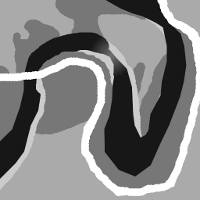
\includegraphics[width=0.3\columnwidth]{terrain.png}}
  \caption{
    Greyscale representations of the three grid-based graph examples \texttt{zig-zag.adj}, \texttt{maze.adj}, and \texttt{terrain.adj}.
    In the images, white signifies easily traversable regions (edge costs = 1), obstacles are black (non-traversable regions: no vertices or edges exist in those areas).
    Darker areas correspond to areas with higher edge costs.
    Note that the files \texttt{zig-zag.grid}, \texttt{maze.grid}, and \texttt{terrain.grid} contain the same data, but in a textual representation.
  }\label{fig:grid-examples}
\end{figure}



\section{Mandatory Tasks}

\begin{figure}
  \centering
  \fbox{
    \begin{minipage}{0.4\columnwidth}
      \verbatiminput{graph-dump-example-nocost.txt}
  \end{minipage}}
  \hfill
  \fbox{
    \begin{minipage}{0.4\columnwidth}
      \verbatiminput{graph-dump-example-cost.txt}
  \end{minipage}}
  \caption{
    Example output for printing the graph defined in \texttt{cities.adj}.
    On the left, before edge cost parsing.
    On the right, after adding edge cost support to the \texttt{Edge} and \texttt{Graph} classes.
  }\label{fig:graph-dump-example}
\end{figure}

\begin{enumerate}

\item
  Extend the provided \texttt{Graph} class such that it actually creates and stores the vertices it reads from the text file.
  Test your result by writing an application that reads \texttt{cities.adj} and prints the resulting graph on the console.
  Your output should look similar to the example given on the left in figure~\ref{fig:graph-dump-example}.
  
\end{enumerate}



\footnotesize
\bibliographystyle{plain}
\bibliography{bibliography}

\end{document}
